\section{Electric Potential and Fields}

In this lab you will study the electric fields and potentials produced by different charge distributions and how charges respond to the presence of these fields.

\vspace{\baselineskip}

\underline{\textbf{Part 1}} \par
1. Consider placing two point charges on an x-y plane, the first charge, $q_1$, at $(x_1, y_1)$, and the second charge , $q_2$, at $(x_2, y_2)$.

\vspace{\baselineskip}

2. Derive an expression for the electric potential and field at any arbitrary point $(x, y)$ in terms of $q_1, q_2, x_1, x_2, y_1$ and $y_2$.

\vspace{\baselineskip}

3. Choose some reasonable values for $q_1, q_2, x_1, x_2, y_1$ and $y_2$ and make a rough sketch of what you expect the electric potential/field to look like.
Your picture doesn't necessarily have to be correct, but you should include some justification for why your sketch looks the way it does.

\vspace{\baselineskip}

4. Use SageMath to draw the exact electric potential and field using the expression derived above.
Below is an example.

\begin{verbatim}
x, y = var("x y")
g = Graphics()
g += contour_plot(1.5 + 0.2*x*y, (x, -4, 4), (y, -4, 4), fill=False, cmap="jet", labels=True, contours=[0, 1, 2, 3, 4], label_fontsize=14)
g += plot_vector_field((y/2, -x/2) , (x, -4, 4), (y, -4, 4)) 
g.show()
\end{verbatim}

Your final result should look something like the figure below.
Note how you can clearly see the two point charges at $(1, 2)$ and $(2, 1.5)$.

\begin{figure}[H]
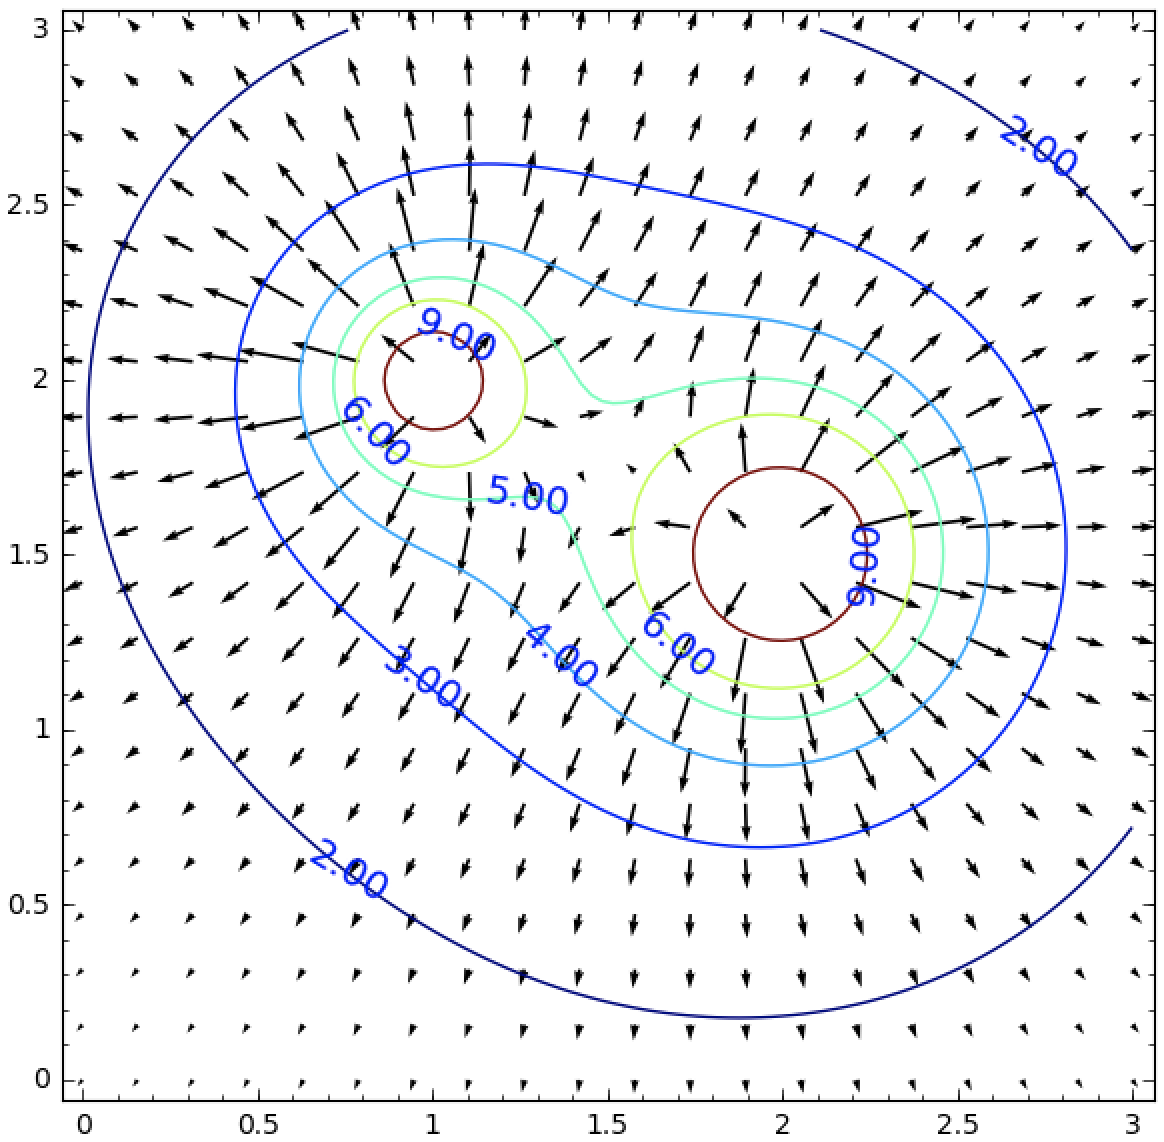
\includegraphics[scale=0.50]{figures/electric-potential-fields/fig1.png}
\end{figure}

\vspace{\baselineskip}

\underline{\textbf{Part 2}} \par

Go to http://www.physicsclassroom.com/PhysicsClassroom/media/interactive/Electric\%20Field\%20Hockey/index.html and complete levels 1, 2, 3, and 5.
Include screenshots in your lab report.

\pagebreak \clearpage
